\documentclass{standalone}
\usepackage{tikz}
\usetikzlibrary{shapes}
\usepackage{tikzpeople}

\begin{document}

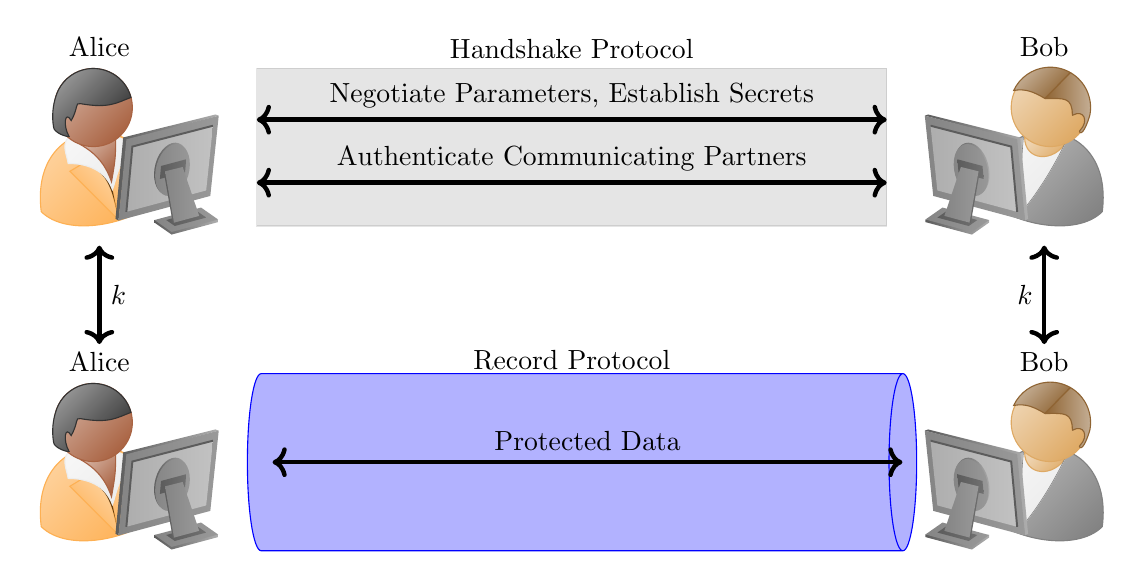
\begin{tikzpicture}
\tikzset{
	cylinder/.style={draw,
		shape=cylinder,
		name=nodename, % Can be defined arbitrarily
		alias=cyl, % Will be used by the ellipse to reference the cylinder
		aspect=1.5,
		minimum height=8.5cm,
		minimum width=2.25cm,
		color=blue,
		fill= blue!30,
		outer sep=-0.5\pgflinewidth, % to make sure the ellipse does not draw over the lines
		%shape border rotate=90
}}
\node[cylinder] (CHANNEL) at (6,0) {};
\draw[draw=black,fill=black, opacity=0.1] (2,5) rectangle  (10,3);
\node[] (HSKLBL) at (6,5.25) {Handshake Protocol};
\node[alice, monitor, label=Alice, minimum size=1.5cm] (Alice) at (0,0) {};
\node[bob, mirrored, monitor, label=Bob, minimum size=1.5cm] (Bob) at (12,0) {};
\node[alice, monitor, label=Alice, minimum size=1.5cm] (Alice) at (0,4) {};
\node[bob, mirrored, monitor, label=Bob, minimum size=1.5cm] (Bob) at (12,4) {};
\node[] (RECLBL) at (6,1.3) {Record Protocol};
{\draw[<->, ultra thick] (2,4.35)  -- (10,4.35) node[midway, above] {Negotiate Parameters, Establish Secrets};}
{\draw[<->, ultra thick] (2,3.55)  -- (10,3.55) node[midway, above] {Authenticate Communicating Partners};}
{\draw[<->, ultra thick] (12,2.75)  -- (12,1.5) node[midway,left] {$k$};}
{\draw[<->, ultra thick] (0,2.75)  -- (0,1.5) node[midway, right] {$k$};}
{\draw[<->, ultra thick] (2.2,0)  -- (10.2,0) node[midway, above] {Protected Data};}

\end{tikzpicture}


\end{document}
